
\chapter{Steganography methods}


\section{Least Significant Bit(LSB)}
\begin{multicols*}{2}
\subsection{Sequential}
\setlength\columnsep{20pt}

Least Significant Bit or LSB is by far the most used method when talking about any type of steganography. Given that the smallest unit a computer can understand and process is usually a byte, altering only the least significant bit will not change the transmitted information in a noticeable way to any external parties. It is much easier to showcase what a byte contains and what the LSB change implies and how it works. A byte contains 8 bits, so this means that the values a byte can take range anywhere from 0 to 255 (inclusive)\footnote{This is the case for unsigned bytes, but given that we are talking about a method that only deals with the least significant bit, we can safely ignore the most significant bit, also known as the sign bit.}. Let's assume that we have an array of 4 random values in consecutive memory : 217, 127, 100, 62 (all values are in decimal), each stored on exactly one byte, and that we want to hide our grade in Numerical Analysis from our parents (in this case a 3) using a LSB substitution. The process would be something like this :

\begin{figure}[H]
    \centering
    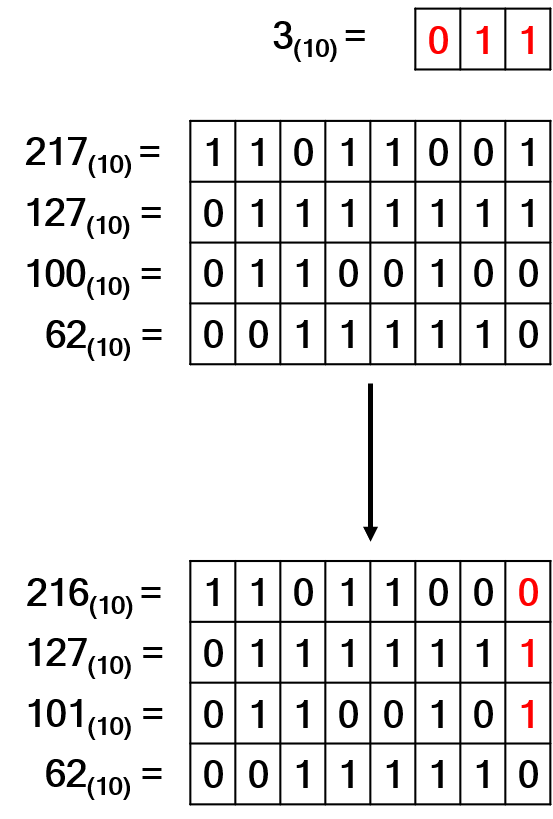
\includegraphics[width=2.8cm,keepaspectratio]{pics/how_lsb_works}
    \caption{How the Least Significant Bit change works}
    \label{LSB}
\end{figure}

As we can see from Figure 2.1, we have succesfully altered the least significant bit of the first 3 bytes of the stream in order to hide our grade : 217 became 216 when we changed the last bit from 1 to 0, 127 was unchanged because it already had the last bit set, and the third byte became 101 after toggling the final bit. Furthermore, the rest of the stream (the fourth byte, 62) was not affected because we already hid the entirety of our secret message. While this is great because we only hide exactly as much as we need and not a byte more, we have a high risk of corrupting the hidden message in case our cover image gets compressed or loses even a single byte when sent over a network. Basically, we are trading data redundancy in order to get simplicity and efficiency.

Sequential LSB insertion is the simplest and most common way of embedding any kind of information into a byte stream that is then shared. It has been thoroughly discussed by a great deal of researchers and has been the subject of many papers where it was analyzed and benchmarked\cite{seeing-the-unseen}\cite{hide-and-seek} . Being the most popular technique also means that any flaws the method has are widely documented and showcased. Steganalysis\footnote{Steganalysis is the study of steganographic methods, including but not limited to : differences in file sizes or in color histograms, secret message redundancy, embedding capacity and performance etc.} performed on outputs created using this algorithm has shown that it is unreliable to stay undetected if an outside party intercepted the message containing the cover file\cite{attack-on-steganography}. Furthermore, doing a simple reverse engineering on the algorithm reveals even more issues with this naive encoding : if a single bit that is part of the secret message was flipped from the cover file byte stream, the message would become corrupted and the original secret would be lost forever. This means that sequential LSB insertion is not resistant at all to any form of lossy compression where some of the original data may be lost in order to reduce the used disk space because it would lose most, if not all, of the embedded file information. 

\subsection{Scrambling}
As documented earlier, sequential LSB insertion algorithm has a decent number of flaws so it was needed to develop some new techniques that are not relying as much on the cover file not losing a few bytes or undergoing a compression algorithm. In other words, it needed to introduce a few redundancies to ensure that the secret message wouldn't be lost as easily. They achieved this by not just changing the least significant bit in a sequential order, but by writing in an apparently random order (in simpler terms, scrambling) that could be reproduced by having the right key or by using the same algorithm in order to retrieve the embedded information. In this subsection we will discuss a few of the most common scrambling techniques and introduce a new one as well.

%research 2 scrambling methods on sci hub, gotta actually read PepeHands

The new algorithm introduced in this paper by the author is a variation of least significant bit insertion that only works on lossless image formats that do not use any kind of interlacing when rendering the picture. It relies on scrambling the secret message into the image sub-blocks in a specific order that can only be deduced by having the right passkey. More information on this method is presented in chapter 3.2.1 after the introduction of image abstracts.
\end{multicols*}

\section{Metadata encoding}


\section{Unused space embedding}
